\section{Теория ридберговских атомов}
\label{sec:Chapter1} \index{Chapter1}


Ридберговские атомы -- это водородоподобные атомы, валентный электрон которых может находиться на высоковозбуждённых уровнях с главным квантовым числом $n \sim 10^2 - 10^3$.
Из теории атома водорода известно, что радиус орбиты электрона возрастает как квадрат главного квантового числа: $r = a_0 \cdot n^2$, где $a_0$ - боровский радиус.
Это приводит к тому, что эффективный размер ридберговского атома в возбуждённом состоянии достигает микрометров, позволяя наблюдать квантовую запутанность и сложную эволюцию систем из таких объектов. 

Данная глава посвящена выводу гамильтониана системы ридберговских атомов и описанию физической реализации квантового устройства.

\subsection{Практическая реализация} \label{seс:aquila}
Хорошим примером платформы для построения моделей квантового машинного служит квантовое устройство на нейтральных атомах Aquila, разработанное Quera \cite{wurtz2023aquila}.
Физическими кубитами данного девайса являются атомы Rb-87, в которые квантовая информация кодируется с использованием орбиталей валентного электрона.
На рисунке \ref{fig:rydberg_atom_spectrum} представлена упрощённая электронная конфигурация данного атома. Фиолетовые линии отвечают за состояния кубита, 
в то время как состояния, отмеченные зелёными линиями, используются для различных манипуляций.

\begin{figure}[htbp]
    \centering
    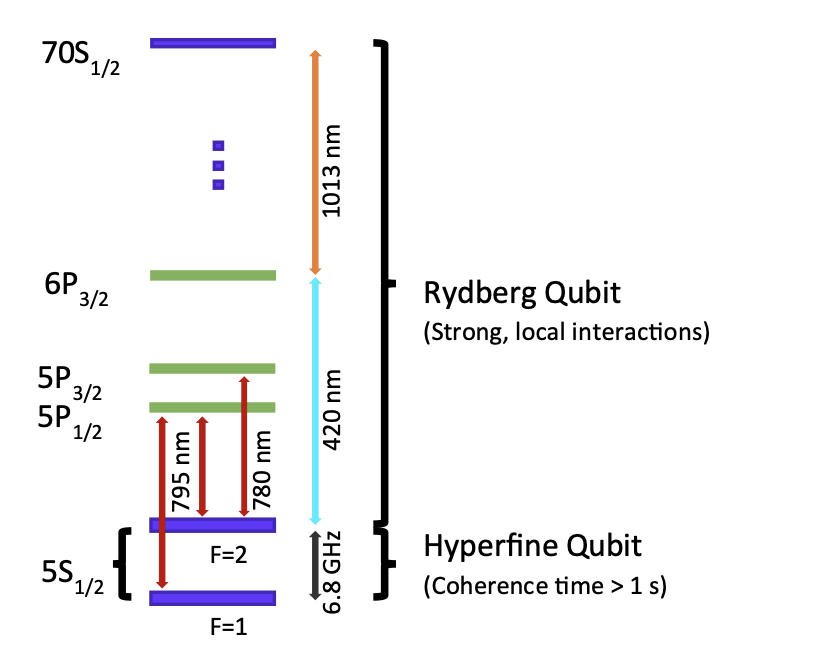
\includegraphics[width=1\linewidth]{images/rydberg_atom_spectrum.png}
    \caption{Состояния валентного электрона атома Rb-87~\cite{wurtz2023aquila}}
    \label{fig:rydberg_atom_spectrum}
\end{figure}

Существуют два набора состояний, на основе которых можно построить двухуровненвую квантовую систему: основный и сверхтонкий ридберговский кубит. 
Сверхтонкий кубит представляется двумя нижними фиолетовыми состояниями:
\begin{equation*}
    \ket{0} = \ket{5S_{1/2}, F=1}, \hspace{3mm} \ket{1} = \ket{5S_{1/2}, F=2}.
\end{equation*}
Данный кубит практически не подвержен взаимодейсвтию с окружающей средой и другими кубитами, а также имеет экстремально длительное 
время когерентности ($\approx$ 1 секунда). Однако современная реализация Aquila работает исключительно в аналоговом режиме и оперирует основными ридберговскими
кубитами с базисом состояний:
\begin{equation} \label{eqn:qubit_states}
    \ket{0} = \ket{5 S_{1/2}}, \hspace{3mm} \ket{1} = \ket{70 S_{1/2}}.
\end{equation}
Такой выбор объясняется тем, что, несмотря на короткое время жизни, возбуждённый уровень валентного электрона представляет собой ридберговское состояние, 
характеризующееся сильным взаимодействием с другими атомами. Данное взаимодействие подробно описывается в секции ~\ref{sec:rydberg_interaction}.


Все атомы находятся внутри стеклянной вакуумной ячейки. Aquila предоставляет возможность захватывать и перемещать отдельные нейтральные
атомы с помощью оптических пинцетов~\cite{ashkin1986tweezers} --- сильно сфокусированных лазерных пучков, расстроенных ниже резонансного перехода
атома рубидия в состояние $6P_{3/2}$. При взаимодействии с неоднородным полем у атома индуцируется дипольный момент, а градиент интенсивности создаёт
силу, удерживающую атом в фокусе пучка. Управление положением атомов осуществляется акусто-оптическими дефлекторами или
пространственными модуляторами света. Параллельно отдельный набор лазеров оптически охлаждает атомы, инициализируя каждый атом в основное состояние.
Такой механизм позволяет создавать практически произвольные двумерные конфигурации атомов, задавая расстояния между ними и, следовательно,
силу ван-дер-ваальсовского взаимодействия. На рисунке~\ref{fig:atom_configurations} представлены примеры таких конфигураций.

\begin{figure}[htbp]
    \centering
    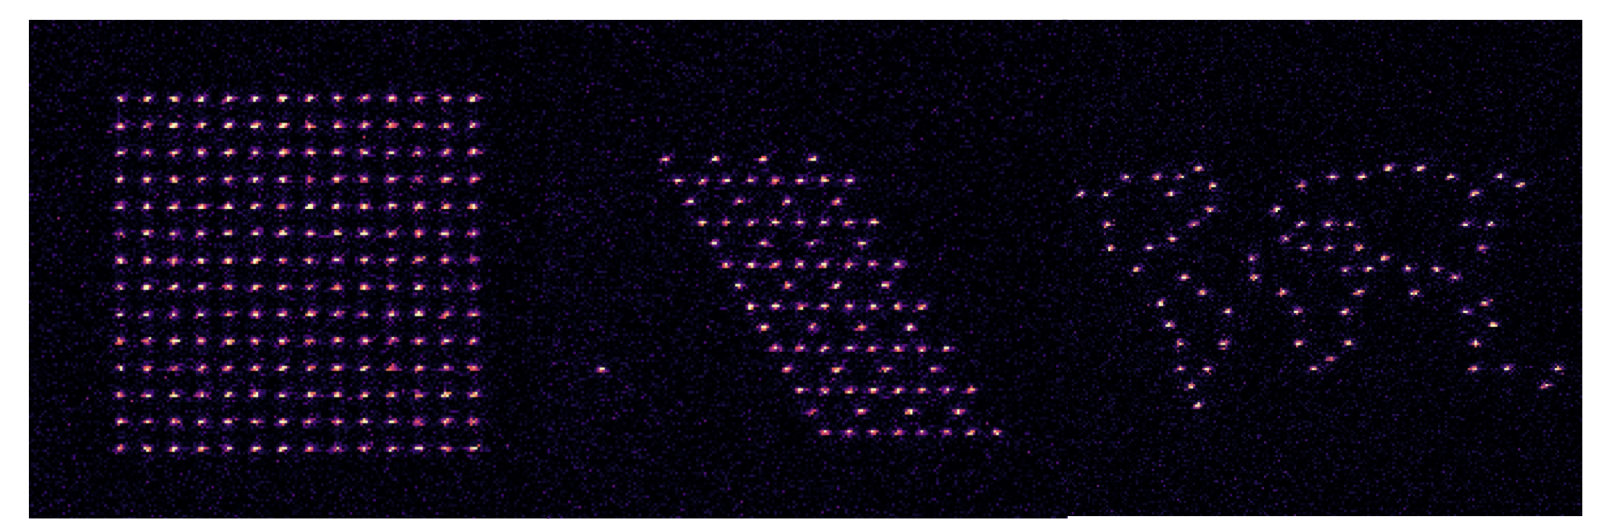
\includegraphics[width=1\linewidth]{images/atom_configurations.png}
    \caption{Примеры двумерных конфигураций массивов нейтральных атомов, реализуемых в устройстве Aquila с помощью оптических пинцетов~\cite{wurtz2023aquila}}
    \label{fig:atom_configurations}
\end{figure}


Измерения в устройстве Aquila производятся методом флуоресцентного детектирования~\cite{bakr2009microscope}.
Во время квантовой эволюции оптические пинцеты отключены и не влияют на динамику системы.
После завершения эволюции пинцеты включаются повторно: атомы в основном состоянии $\ket{0}$ перезахватываются, тогда как атомы
в ридберговском состоянии $\ket{1}$ не захватываются и покидают ловушку.
Последующее флуоресцентное детектирование определяет, в каких ячейках присутствует атом: наличие атома
интерпретируется как состояние $\ket{0}$, отсутствие~--- как $\ket{1}$.
Поскольку атомы в ридберговском состоянии теряются в процессе измерения, оно является разрушающим, и для каждого нового
эксперимента конфигурацию атомов необходимо формировать заново.
С точки зрения квантовой информации данная процедура эквивалентна проекционному измерению в Z-базисе для каждого кубита.

\subsection{Гамильтониан одного атома}
Управление квантовой эволюцией атома производится с помощью специального набора лазеров. В качестве разумного модельного представления 
рассматриваем атом как двухуровневую систему с состояниями \ref{eqn:qubit_states}, связанную с электрическим полем управляющего лазера
$E(t)$ посредством дипольного взаимодействия. Здесь и далее полагаем систему единиц, в которой $\hbar = 1$. Тогда гамильтониан кубита:
\begin{equation}\label{eqn:atom_hamiltonian}
    \hat{H}_a = - \hat{\vec{d}} \vec{E}(t) + (\omega_{1} - \omega_0) \ket{1} \bra{1},
\end{equation}
где $\omega_i$ -- частоты соответствующих состояний атома, $\hat{\vec{d}}$ оператор его дипольного момента.
Первое слагаемое отвечает за дипольное взаимодействие, а второе описывает разность энергий между возбуждённым и основным состоянием.
Исследуем подробнее гамильтониан дипольного взаимодействия:
\begin{equation}
    \hat{H}_d = - \hat{\vec{d}} \vec{E}(t).
\end{equation}
Для дальнейших выкладок удобно ввести обозначение для матричных элементов оператора дипольного момента:
\begin{equation}
    \vec{d}_{ij} = -e\bra{i}\hat{\vec{r}}\ket{j}.
\end{equation}
Тогда в силу симметрийных соображений:
\begin{equation}
    \vec{d}_{00} = \vec{d}_{11} = 0.
\end{equation}
С другой стороны, данный оператор является наблюдаемым в эксперименте, поэтому его внедиагональные элементы действительны и равны друг другу:
\begin{equation}
    \vec{d}_{01} = \vec{d}_{10}.
\end{equation}
Дополнительно будем считать, что электрическое поле лазера является периодическим:
\begin{equation}
    \vec{E}(t) = \vec{E}_0 \cos (\omega_d t + \varphi).
\end{equation}
Таким образом получаем:
\begin{equation}
    \hat{H}_d = \Omega \left(\ket{0} \bra{1} + \ket{1} \bra{0} \right) \cos (\omega_d t + \varphi),
\end{equation}
где за $\Omega = -\vec{d}_{01} \vec{E}_0$ была обозначена $\textbf{частота Раби}$.

Чтобы сохранять двухуровневость атомной системы, необходимо подбирать несущую частоту излучения лазера близкой к резонансному переходу.
Поэтому на практике зачастую выполнено следующее приближение на параметры системы:
\begin{equation} \label{eqn:rot_wave_assumption}
    \omega_1 - \omega_0 \approx \omega_d \gg \Omega.
\end{equation}
В этом случае полный гамильтониан одного атома содержит быстроосциллирующие члены, которыми можно пренебречь. 
Чтобы выделить их явно, необходимо перейти в систему отсчёта, вращающуюся с частотой $\omega_d$. 

Переход в другую систему отсчёта эквивалентен смене базиса в пространстве состояний квантовой системы.
Получим как преобразуется гамильтониан при смене базиса. Для этого рассмотрим уравнение Шрёдингера:
\begin{equation}
    i \frac{\partial}{\partial t} \ket{\psi} = \hat{H}_a \ket{\psi}.
\end{equation}
Переход между базисами задаётся при помощи унитарного оператора $\hat{U}(t)$: 
\begin{equation}
    \ket{\psi} = \hat{U} (t) \ket{\varphi}, \hspace{2mm} \hat{U}^{\dagger}(t) \hat{U}(t) = 1. 
\end{equation}
Тогда уравнение Шрёдингера в новом базисе:
\begin{equation}
    i \frac{\partial}{\partial t} \ket{\varphi} = \left[\hat{U}^{\dagger}(t) \hat{H}_a\hat{U}(t) - i \hat{U}^{\dagger}(t)\frac{\partial}{\partial t}\hat{U}(t) \right] \ket{\varphi}.
\end{equation}
Из квадратных скобок можно извлечь выражение для преобразованного гамильтониана:
\begin{equation}
    \hat{\tilde{H}}_a = \hat{U}^{\dagger}(t) \hat{H}_a \hat{U}(t) - i \hat{U}^{\dagger}(t)\frac{\partial}{\partial t}\hat{U}(t).
\end{equation}
Выбираем оператор перехода к новому базису в форме, описывающей вращение с частотой $\omega_d$:
\begin{equation}
    \hat{U}(t) = e^{-i \omega_d t \ket{1} \bra{1} } = \ket{0} \bra{0} + e^{-i \omega_d t} \ket{1} \bra{1}.
\end{equation}
Опуская выкладки, выпишем преобразованный гамильтониан из (\ref{eqn:atom_hamiltonian}):
\begin{equation}
    \hat{\tilde{H}}_a = \frac{\Omega}{2}\left[(e^{i \varphi} + e^{-2 i \omega_d t - i \varphi} )\ket{0} \bra{1} + (e^{2 i \omega_d t + i \varphi} + e^{-i \varphi}) \ket{1} \bra{0} \right] - \Delta \ket{1} \bra{1}.
\end{equation}
Здесь введено обозначение для $\textbf{детьюнинга}$ $\Delta = \omega_d + \omega_0 - \omega_1$, который описывает насколько частота лазера отклоняется от резонансного перехода между уровнями валентного электрона в атоме.
С учётом условия (\ref{eqn:rot_wave_assumption}) мы можем откинуть быстроосциллилирующие члены в новом гамильтониане:
\begin{equation}
    \hat{\tilde{H}}_a \approx \frac{\Omega}{2}\left(
    e^{i \varphi} \ket{0} \bra{1} + e^{- i \varphi} \ket{1} \bra{0}\right) - \Delta \ket{1} \bra{1}.
\end{equation}
Окончательно рассмотрим общий случай, когда частота Раби $\Omega(t)$, фаза $\varphi(t)$ и детьюнинг $\Delta(t)$ зависят от времени таким образом, что не успевают значительно изменяться за время $1 / \omega_d$.
Тогда предыдущий вывод остаётся в силе, и гамильтониан одного атома в присутствии управляющего лазера записывается в виде:
\begin{equation}
    \hat{\tilde{H}}_a  = \frac{\Omega(t)}{2}\left(
    e^{i \varphi(t)} \ket{0} \bra{1} + e^{- i \varphi(t)} \ket{1} \bra{0}\right) - \Delta(t) \ket{1} \bra{1}.
\end{equation}

\subsection{Взаимодействие Ридберговских Атомов}
\label{sec:rydberg_interaction}


В возбуждённом состоянии валентный электрон ридберговского атома обладает крайне большим главным квантовым числом $n$.
С точки зрения взаимодействия с окружающей системой, главной характеристикой такого возбуждения является колоссальное возрастание поляризуемости атома $\alpha = \frac{|\vec{d}|}{|\vec{E}|}$,
которая асимптотически меняется как $\alpha \sim n^7$~\cite{gallagher1994rydberg}.
Большая поляризуемость означает большие матричные элементы оператора дипольного момента,
поэтому в мультипольном разложении взаимодействия именно дипольный член даёт доминирующий вклад.

Хорошо известно, что взаимодействие двух диполей в лидирующем приближении зависит от расстояния $R$ между ними как $\sim 1 / R^3$.
Здесь имеется в виду ситуация, когда валентные электроны обоих атомов возбуждены.
Однако, если раздвинуть два ридберговских атома на расстояние больше так нызвываемого радиуса Ле Роя \cite{leroy1974},
то характер взаимодействия изменяется -- оно становится ван-дер-ваальсовским.
Не вдаваясь в детальным вывод этого результата и отсылая читателей к \cite{saffman2010quantum}, запишем вид потенцила:

\begin{equation}\label{eqn:van_der_waals_interaction}
    V(\vec{r}_i, \vec{r}_j) = \frac{C_6}{|\vec{r}_i - \vec{r}_j|^6},
\end{equation}
где $C_6$ -- коэффициент ван-дер-ваальса, который измеряется для конкретного сорта атомов на эксперименте.

Как уже отмечалось, данное сильное взаимодействие возникает только в том случае, когда оба атома находятся в возбуждённом (ридберговском) состоянии.
На математическом языке это выражается в следующем вкладе в гамильтониан:
\begin{equation}
    \hat{V}_{ij} = \frac{C_6}{|\vec{r}_i - \vec{r}_j|^6} \hat{n}_i \hat{n}_j.
\end{equation}
Здесь $\hat{n}_i = \ket{1}_i \bra{1}_i$ -- проектор на ридберговское состояние $i$-го атома. 
В контексте квантовых вычислений, именно это взаимодействие ответственно за квантовую запутанность и оно же лежит в основе механизма Ридберговской блокады,
о которой будет идти речь в пункте~\ref{sec:bloqade}.


\subsection{Многочастичный гамильтониан}
\label{seс:manybody_hamiltonian}
Складывая вместе полученные ранее вклады в энергию для каждого атома приходим к общему гамильтониану всей системы:
\begin{equation}
    \hat{H} = \frac{\Omega(t)}{2} \sum_{i} \left(e^{i \varphi(t)} \ket{0_i} \bra{1_i} + e^{-i \varphi(t)} \ket{1_i} \bra{0_i} \right) - \Delta(t) \sum_i \hat{n}_i + \sum_{i < j} \frac{C_6}{|\vec{r}_i - \vec{r}_j|^6} \hat{n}_i \hat{n}_j.
\end{equation}

Заметим, что в приведённом выражении детьюнинг $\Delta(t)$ одинаков для всех атомов системы -- он определяется частотой глобального управляющего лазера.
Тем не менее современная реализация Aquila~\cite{wurtz2023aquila} поддерживает дополнительный канал управления -- локальный детьюнинг,
реализованный посредством отдельного пространственно-неоднородного лазера.

С точки зрения гамильтониана данный лазер создаёт штарковский сдвиг энергии ридберговского состояния каждого атома.
В рамках того же вращающегося представления, что использовалось ранее, вклад этого лазера добавляет в гамильтониан член вида
$-\sum_i h_i \, \delta(t) \, \hat{n}_i$, где $h_i \in [0, 1]$ -- статическая пространственная маска, задаваемая до начала эволюции
(определяет, какая доля локального детьюнинга приходится на $i$-й атом), а $\delta(t)$ -- общая для всех атомов временная огибающая локального детьюнинга.
Суммируя оба вклада, получаем эффективный детьюнинг $i$-го атома:
\begin{equation}
    \Delta_i(t) = \Delta_{\mathrm{global}}(t) + h_i \cdot \delta(t).
\end{equation}
Аппаратные ограничения устройства Aquila накладывают следующие условия на эти параметры~\cite{wurtz2023aquila}:
\begin{itemize}
    \item глобальный детьюнинг $\Delta_{\mathrm{global}}(t)$ может принимать произвольные значения в диапазоне $[-125,\, 125]$ рад/мкс;
    \item временная огибающая локального детьюнинга должна быть неположительной: $\delta(t) \leq 0$, и обращаться в нуль в начале и конце эволюции;
    \item пространственная маска $h_i \in [0, 1]$ является статической на всём протяжении эволюции.
\end{itemize}
Таким образом, подставляя $\Delta_i(t)$ вместо глобального $\Delta(t)$, получаем окончательный вид многочастичного гамильтониана системы ридберговских атомов:

\begin{equation}
    \hat{H} = \frac{\Omega(t)}{2} \sum_{i} \left(e^{i \varphi(t)} \ket{0_i} \bra{1_i} + e^{-i \varphi(t)} \ket{1_i} \bra{0_i} \right) -  \sum_i \Delta_i(t) \hat{n}_i + \sum_{i < j} \frac{C_6}{|\vec{r}_i - \vec{r}_j|^6} \hat{n}_i \hat{n}_j.
\end{equation}
